\newpage
\section{Specyfikacja zewnętrzna}

\subsection{Gra Pong}

Po pomyślnej instalacji serwera wraz z komponentem gry Pong, i otworzeniu zadanej strony w przeglądarce internetowej, na ekranie można będzie zobaczyć widok zapraszający do wzięcia udziału w grze (patrz rysunek ~\ref{fig:mobile_screens}). 
\begin{figure}
\begin{center}
	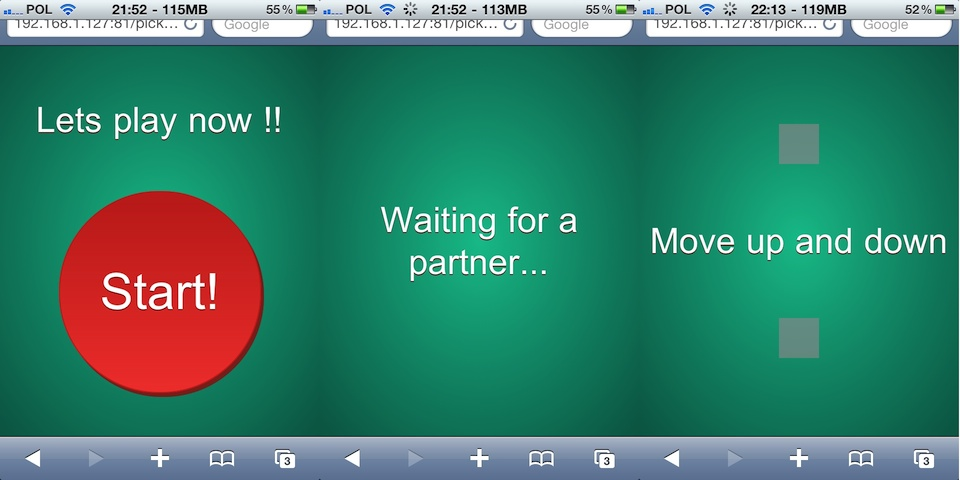
\includegraphics[width=\linewidth]{mobile_screens}
\end{center}
\caption{Zrzut ekranów pokazujący kolejne stany aplikacji od strony klienta}
\label{fig:mobile_screens}
\end{figure}

Po naciśnięciu przycisku Start, klient trafia do kolejki gry, jeśli istnieje możliwość podłączenia się do którejś z trwających gier, to klient zostaje przekierowany do kolejki oczekiwania odpowiedniego serwera. Następnie klient czeka na partnera do gry (co pokazuje drugi widok na rysunku ~\ref{fig:mobile_screens}), lub natychmiastowo zostaje przekierowany do gry i oczom ukazuję się gra której widok został przedstawiony na trzecim zrzucie ekranu. Całym zamysłem gry jest to, że tylko sterowanie grą odbywa się z przeglądarki internetowej klienta, natomiast przebieg gry można obserwować na dużym ekranie tak jak to pokazano na rysunku ~\ref{fig:pong-gameplay}

\begin{figure}
\begin{center}
    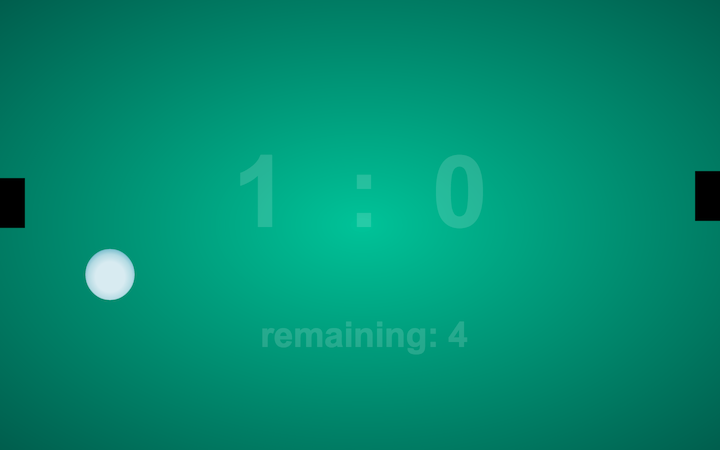
\includegraphics[width=\linewidth]{pong-remote-client-gameplay}
\end{center}
\caption{Zrzut ekranu z trwającej gry}
\label{fig:pong-gameplay}
\end{figure}



\subsection{Aplikacja internetowa zarządzająca infrastrukturą}

Stroną startową aplikacji zarządzającej jest ekran logowania przedstawiony na rysunku ~\ref{fig:managment_login}.

\begin{figure}
\begin{center}
    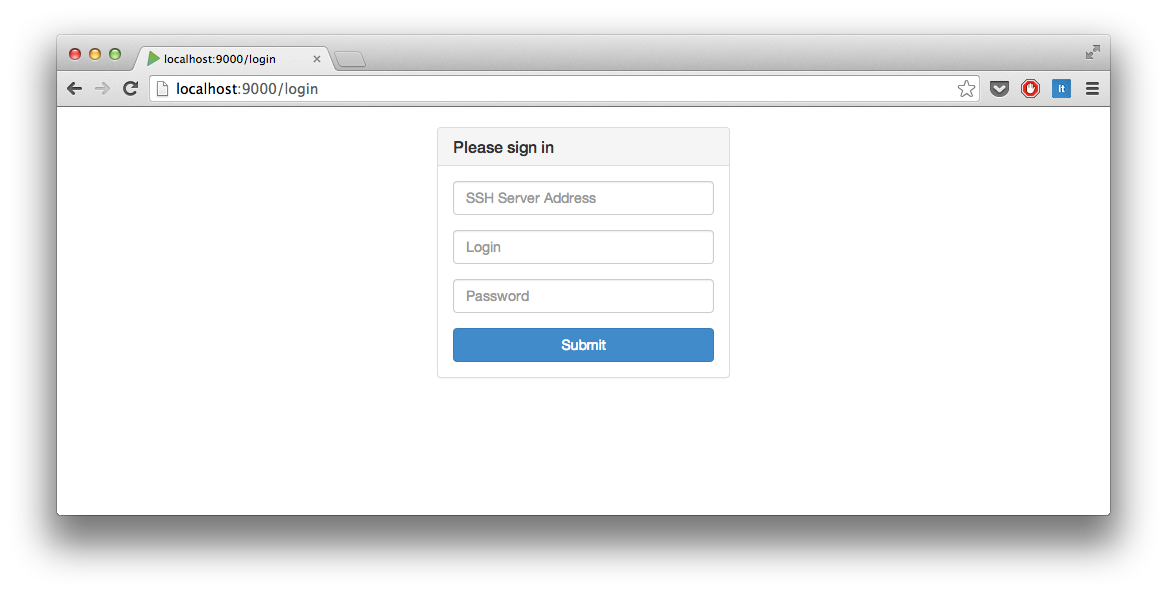
\includegraphics[width=\linewidth]{managment_login}
\end{center}
\caption{Ekran logowania aplikacji zarządzającej infrastrukturą}
\label{fig:managment_login}
\end{figure}

W zakładce Displays istnieje możliwość dodania nowego ekranu po podaniu nazwy, oraz adresu IP wraz z numerem ekranu komputera obsługującego dany wyświetlacz. Po poprawnym dodaniu nowego urządzenia, istnieje możliwość wybrania aplikacji, która będzie wyświetlana na ekranie.

\begin{figure}
\begin{center}
	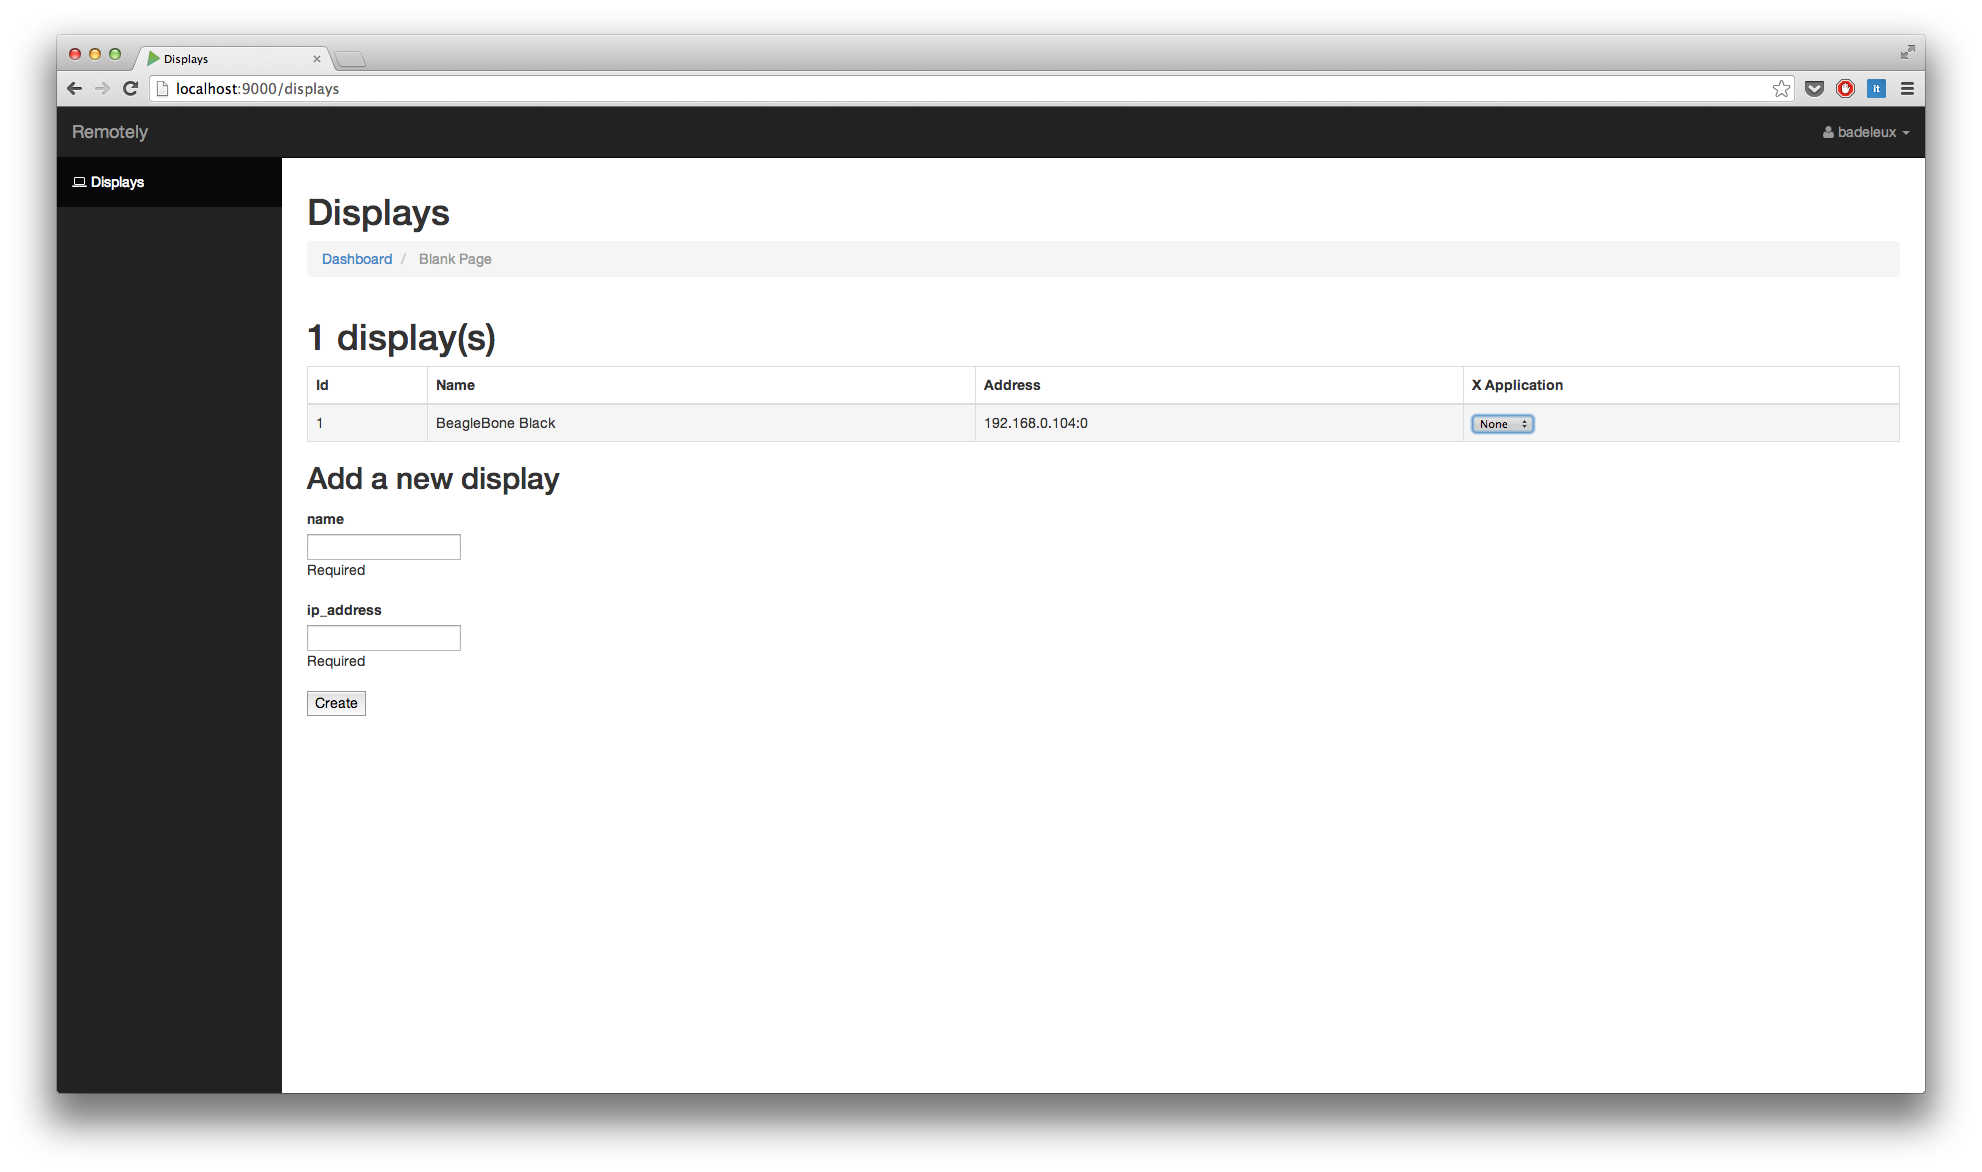
\includegraphics[width=\linewidth]{managment_display}
\end{center}
\caption{Widok zarządzania ekranami}
\label{fig:managment_display}
\end{figure}




